% =======================================================================================
\clearpage
\section{Amortised Cost}
\label{app:amortisation}
% =======================================================================================
% Added 2026-11-19 (user): fit against training time from the cooldown forks, and the number of
% windows after which the flow breaks even with MCMC, with the MCMC time per window a free axis (the
% measured chain times are not those of an optimised pipeline). Numbers from
% paper/scripts/numbers_amortisation.py, figures from fig_amortisation.py.

Training is paid once per band, sampling once per window. This appendix shows how the fit depends on
the training time and after how many windows the training is repaid by the cheaper sampling, which backs
the cost claim of \cref{sec:experiments}.

\paragraph{Fit against training time.}
Each cooldown fork is the same run trained for a shorter schedule (\cref{app:training-loop}): the
forks from epochs 4, 8, 16 and 32 end after 5, 10, 20 and 40 epochs, and cost what a run planned
for that length would. \Cref{fig:amortisation-quality} places them, with the \ResultsEpochs{}-epoch
runs, at the A100 hours of that schedule. On the narrow band, \AmortisationNarrowShortEpochs{}
epochs, \AmortisationNarrowShortHours\,h, already give $f_0$ widths
\AmortisationNarrowShortRatio{} times the chains' at $\snr=15$--40, against
\AmortisationNarrowLongRatio{} after \AmortisationNarrowLongHours\,h; on the full band the same
widths fall from \AmortisationFullShortRatio{} after \AmortisationFullShortHours\,h to
\AmortisationFullLongRatio{} after \AmortisationFullLongHours\,h. The loss falls with training time on every
configuration up to 40 epochs, apart from one step on the full band with $S=4$, and the coverage
stays close to its nominal level throughout, so shorter training gives wider posteriors whose
coverage is unchanged. \textcolor{red}{TODO(trex): check the coverage claim against
fig:amortisation-quality c once built from source-count.json.} The more sources a window holds,
the more training the same width costs. \Cref{tab:results-forks} lists the values.

\begin{figure}[t]
  \centering
  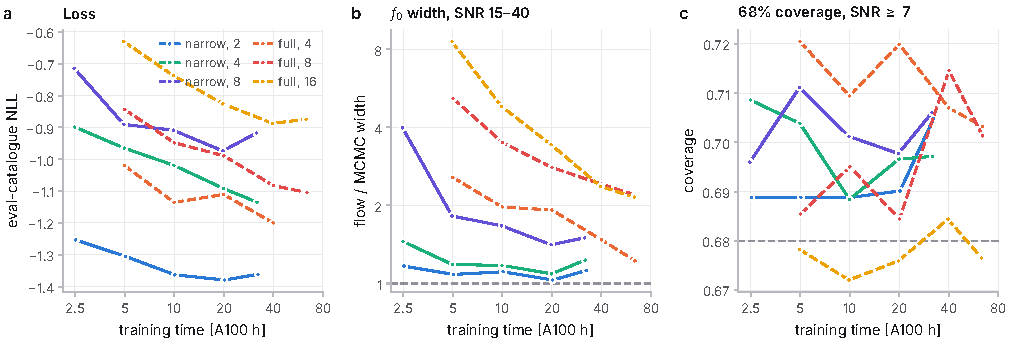
\includegraphics[width=\textwidth]{figures/amortisation-quality.pdf}
  \caption{Fit against training time, for each configuration's cooldown forks (5, 10, 20 and 40
  epochs) and its \ResultsEpochs{}-epoch run (full $S=4$: its Student-t continuation, whose loss does
  not compare and is left out). Training time is the A100 hours of a run planned for that length.
  (a)~Eval-catalogue loss. (b)~Flow over joint-\ac{mcmc} $f_0$ width at $\snr=15$--40, median over the
  sources (\cref{app:results}). (c)~Share of true flow coordinates in the central
  \qty{68}{\percent} interval, pooled over the sources with $\snr\ge7$ and the eight coordinates.}
  \label{fig:amortisation-quality}
\end{figure}

\paragraph{Break-even.}
Let $T$ be the training time, $t_\mathrm{flow}$ the flow's time per window and $t_\mathrm{mcmc}$ the
\ac{mcmc}'s. The flow is cheaper once it has inferred
\begin{equation}
  N^\star = \frac{T}{t_\mathrm{mcmc}-t_\mathrm{flow}}
  \label{eq:amortisation-break-even}
\end{equation}
windows. $t_\mathrm{flow}$ is measured: \AmortisationDraws{} draws take
\qty{\AmortisationNarrowFlowSeconds}{\second} on the narrow band and
\qty{\AmortisationFullFlowSeconds}{\second} on the full band (\cref{app:fm-sampling}). We do not fix
$t_\mathrm{mcmc}$. Our reference chains (\cref{app:mcmc}) were run as an evaluation reference, not tuned
for speed, and a production sampler with tuned proposals, more cores or a GPU likelihood would be faster by a margin
we have not measured. \Cref{fig:amortisation-break-even} therefore shows $N^\star$ against
$t_\mathrm{mcmc}$ from a second to a week. The time axis is wall time on whatever hardware runs the
chains; a different price per hour for the chains' hardware than for an A100 shifts the curves along
it.

As a scale for $N^\star$, one pass over a band infers each frequency once: its windows tiled by
their interiors of \AmortisationInteriorResponses$R$ bins, \num{\AmortisationNarrowPasses} windows
on the narrow band and \num{\AmortisationFullPasses} on the full band. A single pass repays the
training if a chain takes more than \qty{\AmortisationNarrowPassMinutes}{\minute} per window on the
narrow band, or \qty{\AmortisationFullPassMinutes}{\minute} on the full band. If a chain takes an
hour, the flow breaks even after \AmortisationNarrowHourWindows{} and
\AmortisationFullHourWindows{} windows. One pass understates the saving for a global fit, which
revisits each window at every iteration as the neighbouring signals change and starts again with each
data release, while the flow's training is reused as long as the noise model and the priors hold
(\cref{sec:followups}).

\begin{figure}[t]
  \centering
  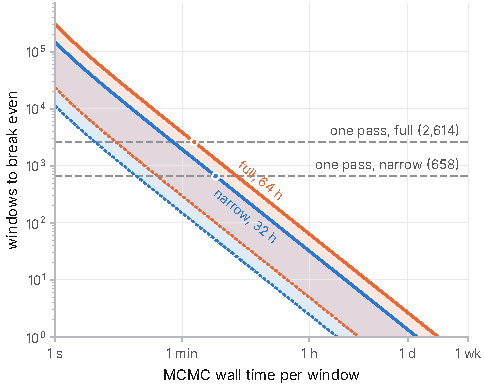
\includegraphics[width=0.5\textwidth]{figures/amortisation-break-even.pdf}
  \caption{Windows after which the flow breaks even with \ac{mcmc}, \cref{eq:amortisation-break-even},
  against the \ac{mcmc} wall time per window. Solid: the \ResultsEpochs{}-epoch runs; dotted: the
  shortest fork (5 epochs); the shading lies between them. Dashed: one pass over each band; the
  dots mark the \ac{mcmc} time at which one pass repays the longest training.}
  \label{fig:amortisation-break-even}
\end{figure}
